\subsection{Android}
The Android component of the system was implemented with the Android 4's design principles in mind. 
This means that the ActionBar has taken over the role traditionally occupied by the menu in previous versions of Android. 
Furthermore, emphasis has shifted away from Activity-centric to Fragment-oriented applications which allows for faster,
 more dynamic and interactive applications. With this in mind it was decided to
 implement the main section of our application as a single activity, called
 HomeActivity, which hosts different tabs for each main view (Product Scanner,
 Product Browser and Shopping List Browser) of our application.
 Each view would then be implemented as a series of Fragments which would move in and out of
 their respective tabs depending on the state of the view. The other views in
 our application (Graph View and Directions View) will be implemented as
 seperate activities which can be launched from our HomeActivity. Unfortunately
 much of this required functionality is not compatible with Android versions
 older than Honeycomb, therefore we needed a workaround. Fortunately this was
 available in the form of ActionBar Sherlock and androidv4, libraries which
 provide us with Android 4 functionality on older versions of Android.  
\subsubsection{Product Scanner}
Not yet implemented.

\subsubsection{Product Browser}
The Product Browser is found in the second tab in our HomeActivity. It was
implemented in the following manner:
\begin{description}
\item[Product Search] This was implemented in two seperate Fragments,
LocationSearchFragment and ProductSearchFragment. LocationSearchFragment allows
the user to specify the locations at which products must be searched for and is
the first Fragment to be displayed in the tab. Clicking on the search button in
it takes the user to the ProductSearchFragment which allows the user to specify
the products or categories to be searched for. Clicking on the search button
here initiates the actual search and takes the user to the BrowseFragment.
\item[Product Viewer] This was implemented as BrowseFragment which displays a
list of the found products. Each list item gives the product's name and price
and is clickable, with a click bringing up an Info Popup. There is also a graph
button present which takes the user to ChartActivity (described in Graph
Viewer).
\item[Info Popup] This was implemented an AlertDialog which displays
information about each product, including:
\begin{itemize}
  \item name,
  \item brand,
  \item size,
  \item price,
  \item date of last scan, and
  \item store scanned at.
\end{itemize} 
The dialog also allows the user to share the product using other applications or
to view the store the product was found at in MapsActivity (described in
Directions Viewer).
\end{description}
\begin{figure}[h!]
\centering
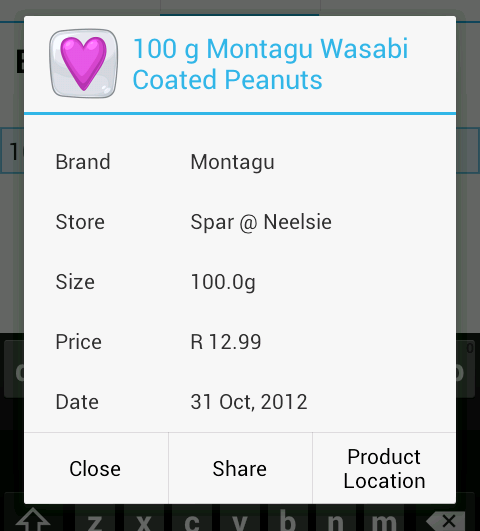
\includegraphics[width=0.3\textwidth]{product-info.png}
\caption{Product info display after a successful search.}
\end{figure}
\subsubsection{Shopping List Browser}
The Shopping List Browser is only partially implemented thus far, with only some of the GUI being designed.
These are the components which have been created:
\begin{description}
\item[ShopScreen] This presents users with a shopping list to which they can add Products.
\item[ShopListAdapter] This is used to display Products on the ShopScreen.
\end{description}

\subsubsection{Graph Viewer}
The Graph Viewer is partially implemented thus far using the following component:
\begin{description}
\item[GraphScreen] This presents users chart for a given dataset.
\end{description}

\subsubsection{Directions Viewer}
The Directions Viewer was implemented using MapsActivity to display our map
and directions in and GoogleParser to request directions from Google's
Directions API and parse so that they can be used in our application. Directions
are displayed in a dialog which can be accessed via a button on the ActionBar
and each intruction can be clicked on which will show the instruction on the
map. 
\begin{figure}[h!]
\centering
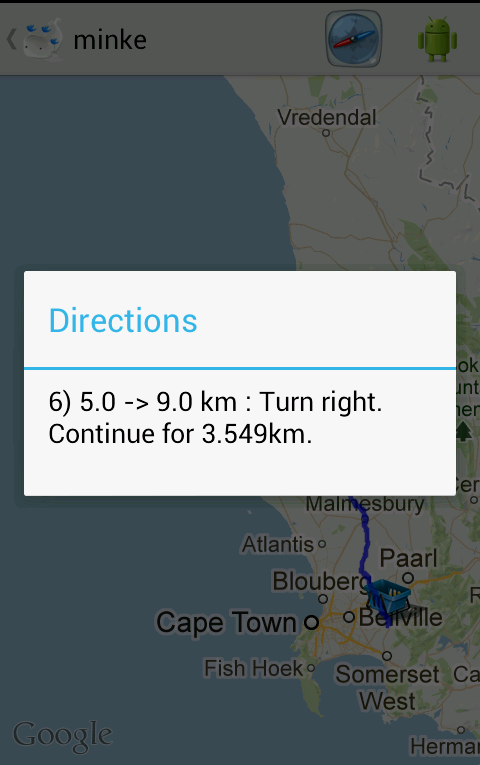
\includegraphics[width=0.3\textwidth]{directions.png}
\caption{Directions view with map.}
\end{figure}
